\documentclass[a4paper,12pt]{article}
\title{Prise de note pour le LAB 3}
\author{Antoine POIRIER}

\usepackage[margin=2cm]{geometry}
\usepackage{graphicx}
\usepackage{float}

\begin{document}

\maketitle

\section*{Les modifications apport\'ees aux fichiers}

\subsection*{Dockerfile}

\begin{center}
	\begin{figure}[H]
		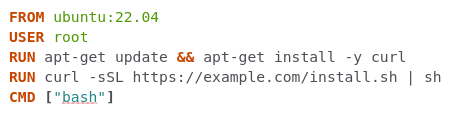
\includegraphics[width=\textwidth]{modif_docker.png}
		\caption{Contenu modifi\'e de Dockerfile}
	\end{figure}
\end{center}

\subsubsection*{Quelle est la r\`egle concern\'ee ?}
La modification que nous avons apport\'e concerne la version de l'image node : on l'a remplac\'e par une version fixe conform\'ement \`a la r\`egle \textbf{CKV\_DOCKER\_7} de l'outil \textbf{checkov}. Cette modification permet \`a l'application conteneuris\'ee de maintenir des d\'ependences stables et de ne pas subir de mises \`a jour cassantes qui pourraient rendre l'application indisponible et demander une intervention des \'equipes op\'erationnelles.

\subsubsection*{Que reste-t-il \`a v\'erifier ?}
Il reste \`a assurer que le conteneur ne soit pas manipulable par des utilisateurs privil\'egi\'es comme ROOT (CKV\_DOCKER\_8). On devrait aussi ajouter des instructions HEALTHCHECK pour surveiller la sant\'e de l'application et r\'eagir rapidement en cas de soucis (CKV\_DOCKER\_2).

\subsection*{deployment.yaml}

\begin{center}
	\begin{figure}[H]
		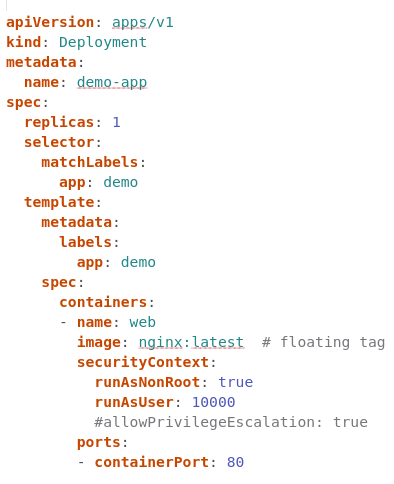
\includegraphics[width=0.5\textwidth]{modif_kubernetes.png}
		\caption{Contenu modifi\'e de deployment.yaml}
	\end{figure}
\end{center}

\subsubsection*{Quelle est la r\`egle concern\'ee ?}
La modification que nous avons apport\'ee est au niveau du champ \textit{securityContext} dans l'objet \textit{containers} : on a fait en sorte que les conteneurs ne puissent \^etre lanc\'es par des utilisateurs privil\`egi\'es. Cette modification concerne la r\`egle \textbf{CKV\_K8S\_23} de l'outil \textbf{checkov}.

\subsubsection*{Que reste-t-il \`a v\'erifier ?}
Les r\`egles \`a v\'erifier sont en lien avec l'UID des utilisateurs \textit{(CKV\_K8S\_40)} et la gestion responsable des ressources comme la m\'emoire \textit{(CKV\_K8S\_12)}.

\subsection*{main.tf}

\begin{center}
	\begin{figure}[H]
		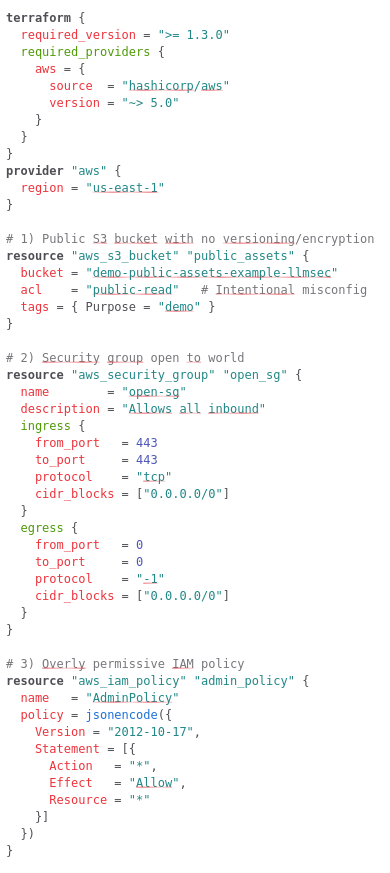
\includegraphics[width=0.5\textwidth]{modif_terraform.png}
		\caption{Contenu modifi\'e de main.tf}
	\end{figure}
\end{center}

\subsubsection*{Quelle est la r\`egle concern\'ee ?}
La r\`egle concer\'ee est \textbf{CKV\_AWS\_25} de l'outil \textbf{checkov}. Cette r\`egle insiste sur l'importance de d\'efinir des security group avec le bon \'equilibre de s\'ecurit\'e et de disponiblit\'e du service. Dans ce cadre-l\`a, nous avons pris la d\'ecision de changer la r\`egle \texttt{ingress} de la ressource \texttt{aws\_security\_group} pour n'accepter que les requ\^etes \`a destination du port 443 \textit{(port habituel pour HTTPS qui est chiffr\'e)} et utilisant le protocole TCP.

\subsubsection*{Que reste-t-il \`a v\'erifier ?}
Il reste \`a prendre en compte des r\`egles en lien avec la description des security group pour l'auditabilit\'e \textit{(CKV\_AWS\_23)}. D'autres concernent la bonne application des r\`egles IAM \textit{(CKV\_AWS\_288)}.

\vspace{1cm}

\begin{center}
	\begin{tabular}{|c|c|c|}
		\hline
		\textbf{fichier} & \textbf{modification} & \textbf{r\`egle concern\'ee} \\
		\hline
		\texttt{Dockerfile} & Version de l'image node fix\'ee \`a 22.04 & CKV\_DOCKER\_7 \\
		\hline
		\texttt{deployment.yaml} & Minimisation de l'abus des privil\`eges & CKV\_K8S\_23 \\
		\hline
		\texttt{main.tf} & Renforcement du groupe de s\'ecurit\'e entrant & CKV\_AWS\_25 \\
		\hline
	\end{tabular}
\end{center}

\end{document}
